\chapter{The Scratch Online Community}

%TODO: once settled with layout, make sure it does not use a full page just for this image
\begin{figure}
\centering
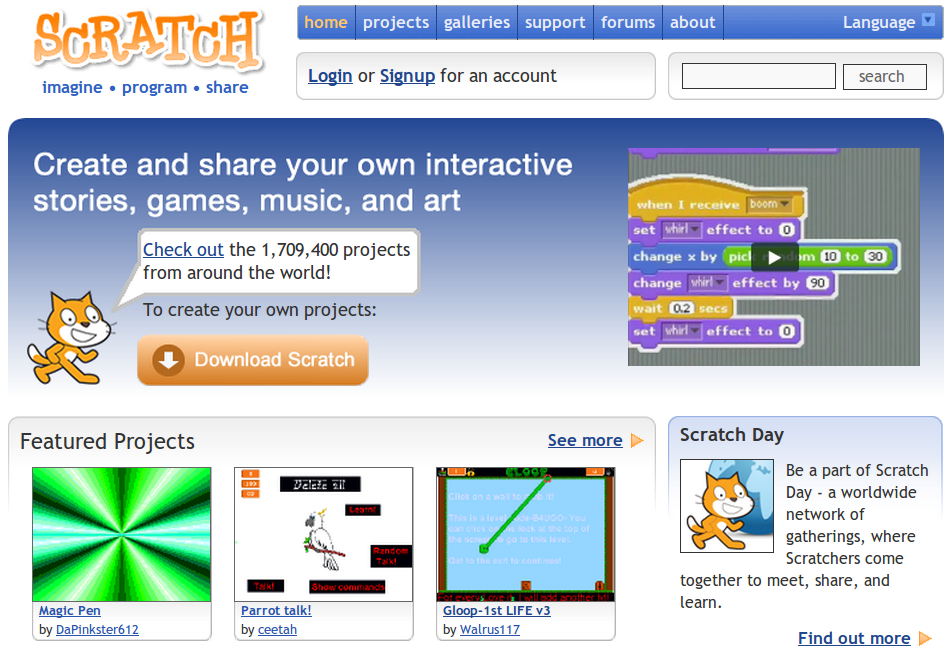
\includegraphics[width=3.25in]{figures/websitehomepage.png}
\caption{The home page of the Scratch website}
\label{fig:websitehomepage}
\end{figure}

The empirical setting for this work is the Scratch Online Community, a website (Figure~\ref{fig:websitehomepage}) I conceived and developed over the past four years in collaboration with others at the Lifelong Kindergarten research group, for this and other lines of research.
The website allows anyone, especially young people between ages eight and sixteen, to share their animated stories, interactive art, and video games. Participants use the Scratch programming environment, a desktop application, to create or remix projects by putting together images, music and sounds with visual programming command blocks \citep{resnick_scratch:_2009}.
Projects range from interactive greeting cards, physics simulations, animations of popular songs to homemade video games, just to name a few.  

Scratch projects are organized in sprites (e.g. a character in a game).
Each sprite has a set of ``costumes'' or images that represent its different visual states, for example, a sprite of a bird flying could have multiple costumes, each one representing the different positions of the wings. 
Sprites can also have sounds associated to them, these sounds can be either recorded with the microphone or imported from the hard creator's hard drive. Finally, sprites' behavior is controlled by ``scripts'' which are stacks of visual programming blocks. 

In my dissertation, I  document in detail the motivations that led to the design of the Scratch website as it is now and the various iterations that it went through as a result of internal and user-driven demands and participation patterns.
I expand on the tight relationship between the technical capabilities of the website and the social dynamics that it supported or intended to support.
I take a critical look at how the original goals of the community were or were not achieved and in what ways that happened. 
I narrate scalability challenges with the technology and moderation of the community.
In the following two sections I provide a glimpse of this.

More broadly, I try to tackle questions such as: How was the culture of sharing seeded and maintained in a public space? What were some important incidents that changed policies or architecture? How did the architecture and management of the site influence the culture of the site and how did users help shap this? 
Was it the design of the space or the work of users to create the culture?
 What were the lessons learned along the way by administrators? What kinds of learning outcomes were achieved?
To answer some of these questions, I primarily rely on participant observation data, experiences collected during the three years and I support these arguments with descriptive statistics and case studies.


\section{Motivations}

From its start \citep{monroy-hernandez_scratchr:_2007,monroy-hernandez_empowering_2008}, I set the goal for the Scratch Online Community as to give creators access to 
1) a \emph{network of peers} that functions as an audience and as potential collaborators and,
2) a \emph{repository} of inspirational creations that can be creatively appropriated by anyone.

More broadly, the Scratch Online Community was created with the idea of supporting a Community of Practice around Scratch where novices and experts would come together,  in the spirit of Papert's Samba school's metaphor \citep{papert_mindstorms_1980}.

Additionally, the idea of the Scratch Online Community was conceived under the umbrella of embodying the ethos of Participatory Culture of empowering people to become producers rather than just consumers of media.

Last, the Scratch Online Community was motivated to support the various iterative stages of the creative process \citep{resnick_sowing_2008}, namely:
Supporting creators' \emph{imagination} by giving access to a pool of inspirational projects and ideas; supporting \emph{creation} by allowing people to reuse and remix; supporting \emph{play} by letting people interact with others and their creations within a community; supporting \emph{sharing} by allowing people to easily upload their creations to the platform; supporting \emph{reflection} by providing a space to receive comments and discussion forums for more in-depth discussions.

\section{Sociotechnical Infrastructure}
The Scratch website platform, called ScratchR, is broadly composed of the following components: 

\begin{enumerate}
\item A repository of projects and metadata. Projects can be downloaded by anyone, modified and re-uploaded to the website as a remix. Each project has its web page where it is displayed and where people can interact with it and other people. 

\item A social network consisting of profile pages and unidirectional friendship connections. Profile pages list the friends, projects and ``favorited'' projects for each user with his or her avatar image and the Country of origin (all self-reported data).

\item Social features for interacting with people's creation such as commenting, tagging, ``loving'', ``favoriting''.

\item Galleries, which are pages where people can group projects and talk about them. It is important to note that galleries have been repurposed by the community as group spaces where people collaborate to create projects or use it as a space to talk to one another or play Role Playing Games.

\item Discussion forums where community members help one another with technical problems, find collaborators and talk about non-Scratch related activities that foster a sense of community on the website.

\item External services supported by an API\footnote{API stands for Application Program Interface. In ScratchR, they are a set of web-accessible functions that let people retrieve and submit data such as login authentication and information about projects.} such as a website where people can link projects or a Wiki where people can document their experiences with Scratch and the community.
\end{enumerate}

The website runs on a hybrid model for moderation that combines user-driven moderation through flagging and appointed moderators working in parallel with a full-time staff member and other part-time ones that review the flags and ensure that the social dynamics are kept as civil as possible. 
This model has allowed for scaling the community management at a relatively low cost, however, much of the architecture and software development during the three years has been put into mechanisms for preventing antisocial behavior.

Three years after its official release, the Scratch Online Community website I developed, handles more than ten million page views and six hundred-thousand people monthly.
This web traffic is more than half the page views of websites like newsweek.com\footnote{04/2011 data from http://www.quantcast.com/newsweek.com}.
As of April of 2011, more than 1.7 million projects have been uploaded at an average of 1 MB per project. 
Every second, the website receives up to 180 requests and it transfers 4MB.

To handle this level of activity, ScratchR, the website's underlying platform, uses a caching engine for static content called Varnish and another for dynamic content and database queries called Memcached. 
ScratchR runs on a completely Free and Open Source software stack that includes Apache for its web server and MySQL for its database running on CentOS Linux. 
ScratchR is written using a PHP-based framework called CakePHP.
Additionally, ScratchR supports external  web applications such as a discussion forum, a user-driven Wiki, a statistics visualization website, a Scratch sprites sharing website, and a few other websites that provide additional support to community members. 
These extra websites are supported through an API that has allowed scalability.

\section{Building an Online Community}

People often ask us how the Scratch Online Community become ``successful.''
Of course, ``success'' is not only relative but can also mean many different things for different people.
Assessing the success of an online community is an rich area of research explored by others \cite{preece_online_2000} and slightly tangential to the goal of this document. 
My goal here is merely to describe how the Scratch Online Community has or has not achieved some of the desired outcomes.
Broadly speaking, I am considering here two versions of success \emph{size} and \emph{engagement}.
\begin{enumerate}
\item Size. The simplest and perhaps most naive measure of success is based on the number of registered users, contributed content, pageviews and visits to a website. 
With close to one million users, two million contributed projects, ten million pageviews and one million visits, the Scratch Online Community is big for an academic research project but quite small compared to other similar online spaces such as YouTube's 14 billion videos \cite{comscore_comscore_2010}.

\item Engagement. A more nuanced and difficult form to assess the success of an online community is by looking at the diversity and richness of its member's interactions.
We have documented some of these rich interactions through stories of members of the online community that show how for many participants, the Scratch Online Community is not only a website where they upload projects but a space where they like to hang out to meet and interact with peers.
\end{enumerate}

It is hard to know exactly what contributed to lead the success of an online community but here I describe the set of broad sociotechnical steps that I think contributed to the success of the Scratch Online Community. I believe that even if they are the result of post-hoc rationalization, they might provide insights to others trying to work on this space.

\begin{enumerate}
% TODO: make sure to go from Scratch to generalizable ideas.
\item High-quality creation tool.
The online community success is undeniably linked to the quality of the Scratch authoring tool.
Members of the Lifelong Kidnergarten Group \footnote{In particular John Maloney, Evelyn Eastmond, Brian Silverman, Paula Bonta and Natalie Rusk with the guidance and leadership of Mitchel Resnick, probably have more than half a century of combined experience developing creative tools for kids}
have spent countless hours over the years perfecting the Scratch programming environment.
Every pixel in the screen has probably had more hours of work than any other aspect of the Scratch experience.
This attention to detail in the Scratch appllication has greatly contributed to the solid user experience of Scratch, even at the expense of agility.

\item Bootstraping. A lot of online social spaces face the problem of adoption.
Others have already described the challenges of benefiting from the network effect \cite{TODO}. 
How does one get people to participate in an online community before there are any users? 
The way I approached this was by seeding the community with participants recruited as part of Scratch workshops. 
I started with an 11-week workshop for underserved middle-schoolers as part of an initiative called Citizen Schools \footnote{
``Citizen Schools partners with middle schools to expand the learning day for children in low-income communities across the country. By drawing thousands more citizens into schools each year, we’re promoting student achievement, transforming schools, and re-imagining education in America.'' http://citizenschools.org}

\item Authentic participation.
For the very beginning I set myself to the task of being an authentic and active member of the community. Everyday, I would browse the website, playing with people's projects and leaving comments giving suggestions or simply describing how and why I enjoyed different aspects of someone's work. 
I think for a lot of kids on the site, knowing that their work is being seen and eliciting responses from others is a big motivation to come back.
% TODO: quote.
I always tried to be aware of representing myself as the caring adult rather and used the language that I would use in my everyday online conversations.
Avoiding complicated language or to be ``one of the kids''. 
I tried to maintain a real profile.

\item Empowering active members.
Early on it was clear that some people were not only spending more time on the site but also contributing to it in really meaningful and positive ways.
Some of them were adults and others were kids.
I tried to acknowledge their presence and recognize when possible by featuring their work on the front page or even inviting some of them to become ``moderators'' of the discussion forums. 
This is an aspect of an online community where technological interventions can be quite effective.

\item Quick iterations.
As mention before, the Scratch desktop application, has been developed in a careful, slow and almost artesanal model that had led to a high-quality product.
The Online Community development took a radically different approach.
Inspired by some of the aspects of Agile software development \cite{TODO}, the website's evolved with its users through quick iterations.
The first version of the website tried to make few assumptions and tried to provide some of the
application had a handful of update in the four years. 
In part because its careful almost artesanal development model that led  difficult to deploy software changes that require people to update but
The online community evolved quickly through a series of continous iterations. On the other hand, the Scratch desktop application was carefully crafted before the online component. The desktop application was the result of years of field experience that became ingrained in the designers' intutions. 

\item Emphasize user contributions.
Layout was maintained simple, perhaps too simple compared to other sites for kids.
There is something to say about simplicity in web design.
Sites like craigslist or 4chan have proved to be quite successful despite having extrmely simply and archaic designs.

\item Software-embodied culture and policies.
Code implements way of thinking.
Lessig.
\item Generalizable specifity.
At the surface, the Scratch Online Community is about sharing animations and video games, however, people come together to do more than that. 
People discuss their family and school lives, the games they like.
Scratch is a place to hang out with like-minded individuals, it's a clubhouse not just a repository.
Online communities need to balance between focusing on something specific (e.g. programming) and letting the conversations diverge into the general (e.g. family issues).
Some of the most successful (in terms of volume and engagement) online communities have exhibited similar patterns of helpful divergence.
For example, reddit.com was originally focused on technology topics and now it has diverged into comics, politics, science and arts.
Similarly, one of the most controversial and influential communities, 4chan, was originally focused on Anime sub-culture and now it has diverged into a similar wide range of topics as reddit.
Likewise, Facebook originally focused on college life and Flickr on sharing screenshots of videogames.
The ``seeding culture'' influences the discourse and the type of people that it attracts, but once it happens, community designers must give some room for divergence. 
How much divergence depends on how much the designers want the community to grow.
As it diverges, it also alineates long-time participants.

\end{enumerate}
